\documentclass[10pt,t]{beamer}\usepackage[]{graphicx}\usepackage[]{color}
%% maxwidth is the original width if it is less than linewidth
%% otherwise use linewidth (to make sure the graphics do not exceed the margin)
\makeatletter
\def\maxwidth{ %
  \ifdim\Gin@nat@width>\linewidth
    \linewidth
  \else
    \Gin@nat@width
  \fi
}
\makeatother

\definecolor{fgcolor}{rgb}{0.345, 0.345, 0.345}
\newcommand{\hlnum}[1]{\textcolor[rgb]{0.686,0.059,0.569}{#1}}%
\newcommand{\hlstr}[1]{\textcolor[rgb]{0.192,0.494,0.8}{#1}}%
\newcommand{\hlcom}[1]{\textcolor[rgb]{0.678,0.584,0.686}{\textit{#1}}}%
\newcommand{\hlopt}[1]{\textcolor[rgb]{0,0,0}{#1}}%
\newcommand{\hlstd}[1]{\textcolor[rgb]{0.345,0.345,0.345}{#1}}%
\newcommand{\hlkwa}[1]{\textcolor[rgb]{0.161,0.373,0.58}{\textbf{#1}}}%
\newcommand{\hlkwb}[1]{\textcolor[rgb]{0.69,0.353,0.396}{#1}}%
\newcommand{\hlkwc}[1]{\textcolor[rgb]{0.333,0.667,0.333}{#1}}%
\newcommand{\hlkwd}[1]{\textcolor[rgb]{0.737,0.353,0.396}{\textbf{#1}}}%
\let\hlipl\hlkwb

\usepackage{framed}
\makeatletter
\newenvironment{kframe}{%
 \def\at@end@of@kframe{}%
 \ifinner\ifhmode%
  \def\at@end@of@kframe{\end{minipage}}%
  \begin{minipage}{\columnwidth}%
 \fi\fi%
 \def\FrameCommand##1{\hskip\@totalleftmargin \hskip-\fboxsep
 \colorbox{shadecolor}{##1}\hskip-\fboxsep
     % There is no \\@totalrightmargin, so:
     \hskip-\linewidth \hskip-\@totalleftmargin \hskip\columnwidth}%
 \MakeFramed {\advance\hsize-\width
   \@totalleftmargin\z@ \linewidth\hsize
   \@setminipage}}%
 {\par\unskip\endMakeFramed%
 \at@end@of@kframe}
\makeatother

\definecolor{shadecolor}{rgb}{.97, .97, .97}
\definecolor{messagecolor}{rgb}{0, 0, 0}
\definecolor{warningcolor}{rgb}{1, 0, 1}
\definecolor{errorcolor}{rgb}{1, 0, 0}
\newenvironment{knitrout}{}{} % an empty environment to be redefined in TeX

\usepackage{alltt}

\usetheme[progressbar=frametitle]{metropolis}

\usepackage{booktabs}
\usepackage{natbib}
\usepackage[scale=2]{ccicons}
\usepackage{lmodern}
\usepackage{ulem}
\renewcommand<>{\sout}[1]{
  \alt#2{\beameroriginal{\sout}{#1}}{#1}
}

%\usepackage{animate}

%\usepackage{xspace}
%\newcommand{\themename}{\textbf{\textsc{metropolis}}\xspace}
%\renewcommand\textbullet{\ensuremath{\bullet}}

\newcommand{\bX}{\mathbf{X}}
\newcommand{\bY}{\mathbf{Y}}
\newcommand{\mat}[1]{\mathbf{#1}}
\renewcommand{\vec}[1]{\boldsymbol{#1}}
\newcommand{\bx}{\mathbf{x}}
\newcommand{\bxi}{\bx^{(i)}}
\newcommand{\bw}{\mathbf{w}}
\newcommand{\bz}{\mathbf{z}}
\newcommand{\bnu}{\boldsymbol{\nu}}

\usepackage{tikz}
\usetikzlibrary{calc,positioning}


\title{Real-time prediction of bus arrival using joint models for vehicle and road state}
%\subtitle{}
\author{Tom Elliott}
\date{}
\institute{Supervisor: Professor Thomas Lumley\\[2em]

\includegraphics[height=1.5cm,width=3.8cm]{stat-logo.png}}

%Department of Statistics\\University of Auckland}
%\titlegraphic{\hfill
\includegraphics[height=1.5cm]{stat-logo.png}}
\IfFileExists{upquote.sty}{\usepackage{upquote}}{}
\begin{document}

\maketitle


\begin{frame}
  \frametitle{Overview}
  
  \begin{enumerate}
  \item A quick motivation
    
  \item Two real-time models: vehicle (particle filter) \& road (Kalman filter)
    
  \item Predicting arrival times
  \end{enumerate}
\end{frame}


\begin{frame}
  \frametitle{What's wrong with the current\footnote{Auckland Transport} system?}
  
  \pause
  \begin{itemize}[<+->]
  \item Prediction inaccuracy
    
  \item Prone to errors
    
  \item<7-> Recent modelling frameworks \emph{don't} make use of 
    all real-time vehicle data
  \end{itemize}
  
  \begin{overprint}
    \onslide<3-6>
    \centering
    \onslide<3->{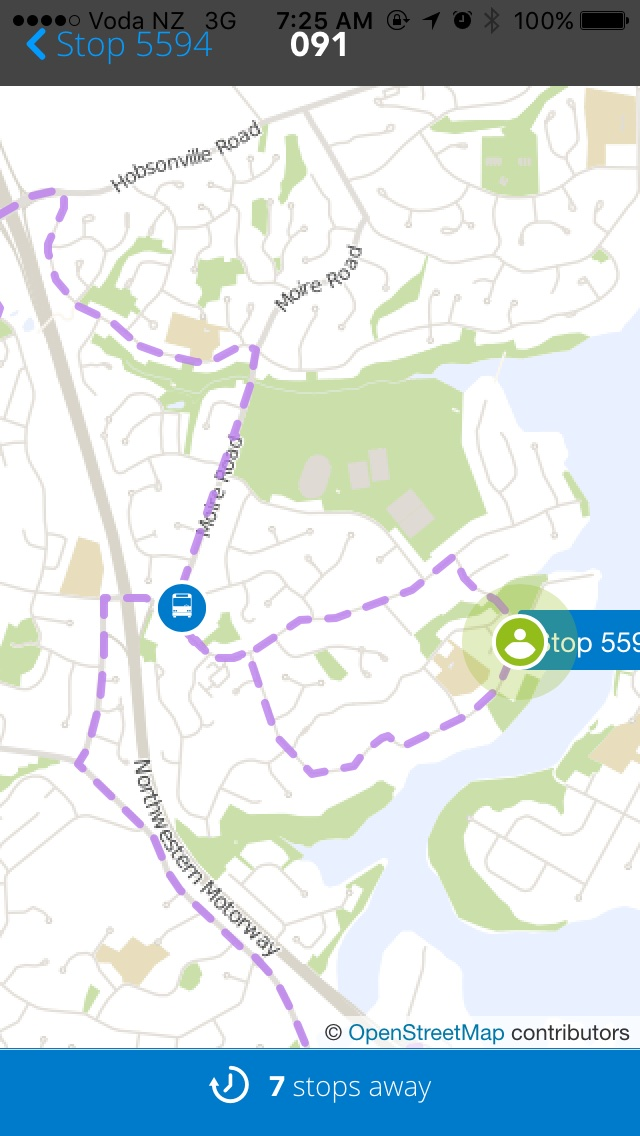
\includegraphics[width=0.2\textwidth]{figure/colwill-1.jpg}\hspace{1em}}
    \onslide<4->{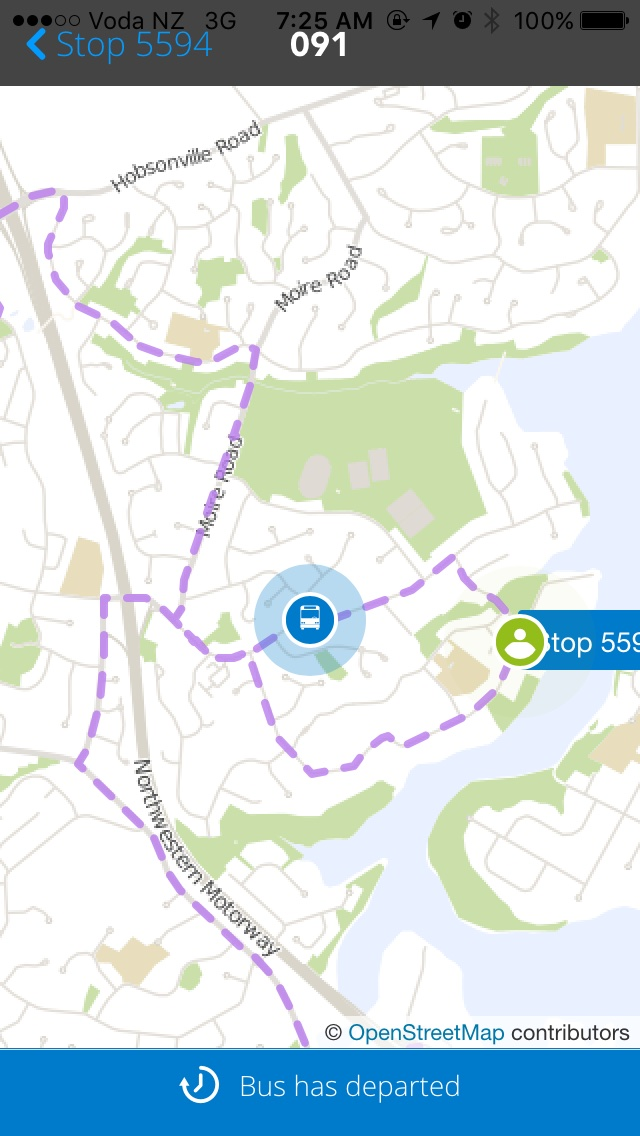
\includegraphics[width=0.2\textwidth]{figure/colwill-2.jpg}\hspace{1em}}
    \onslide<5->{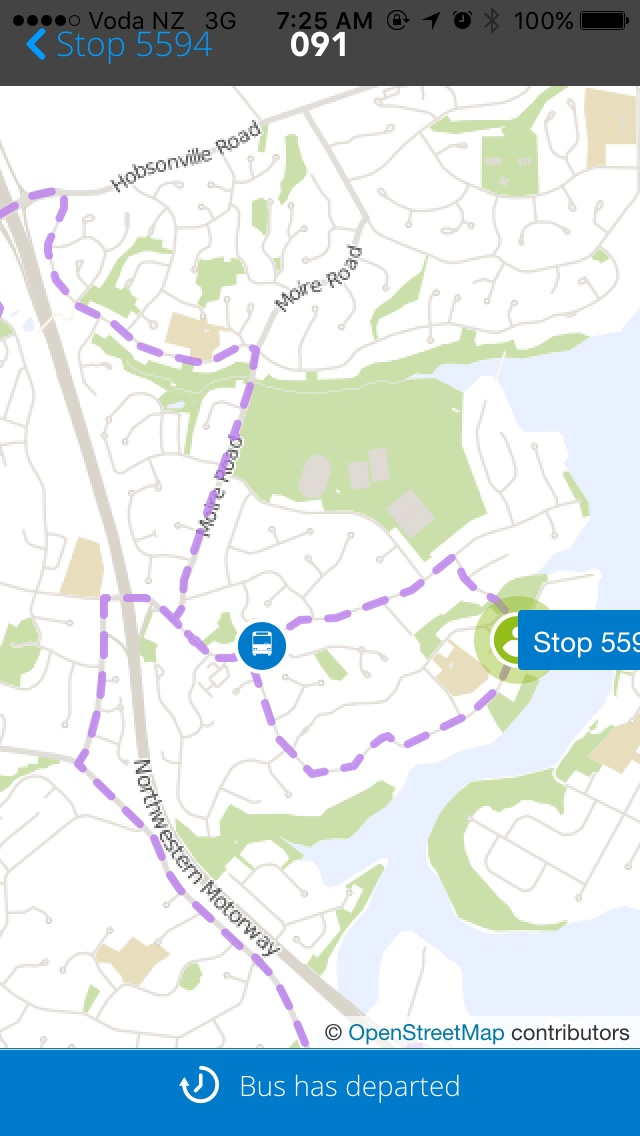
\includegraphics[width=0.2\textwidth]{figure/colwill-3.jpg}\hspace{1em}}
    \onslide<6->{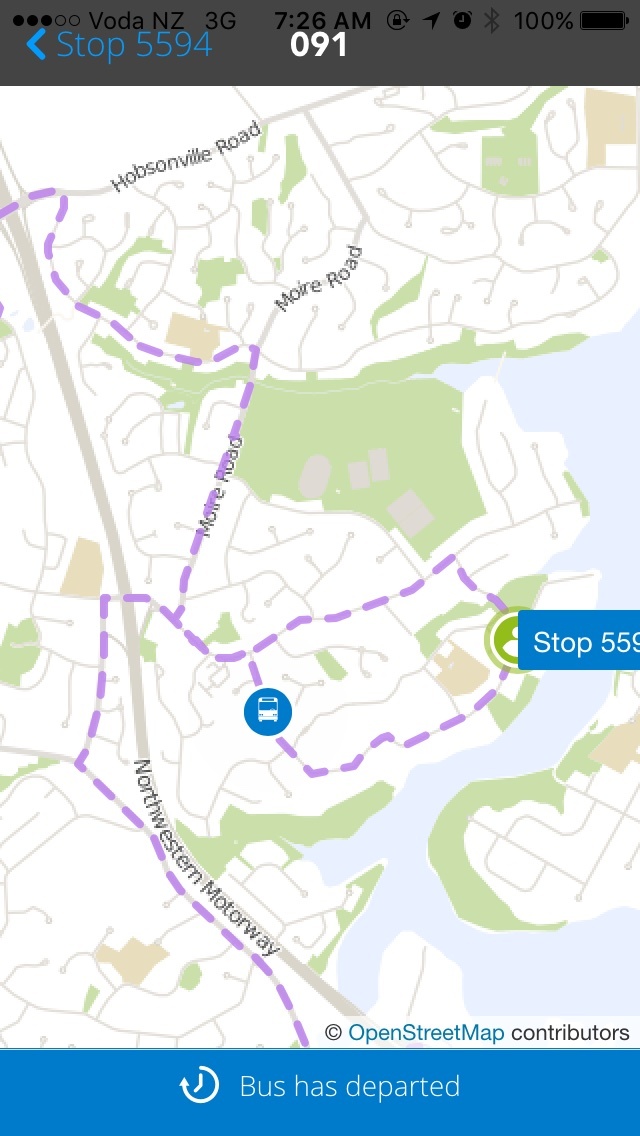
\includegraphics[width=0.2\textwidth]{figure/colwill-4.jpg}}
    
    \onslide<7>
    \centering
    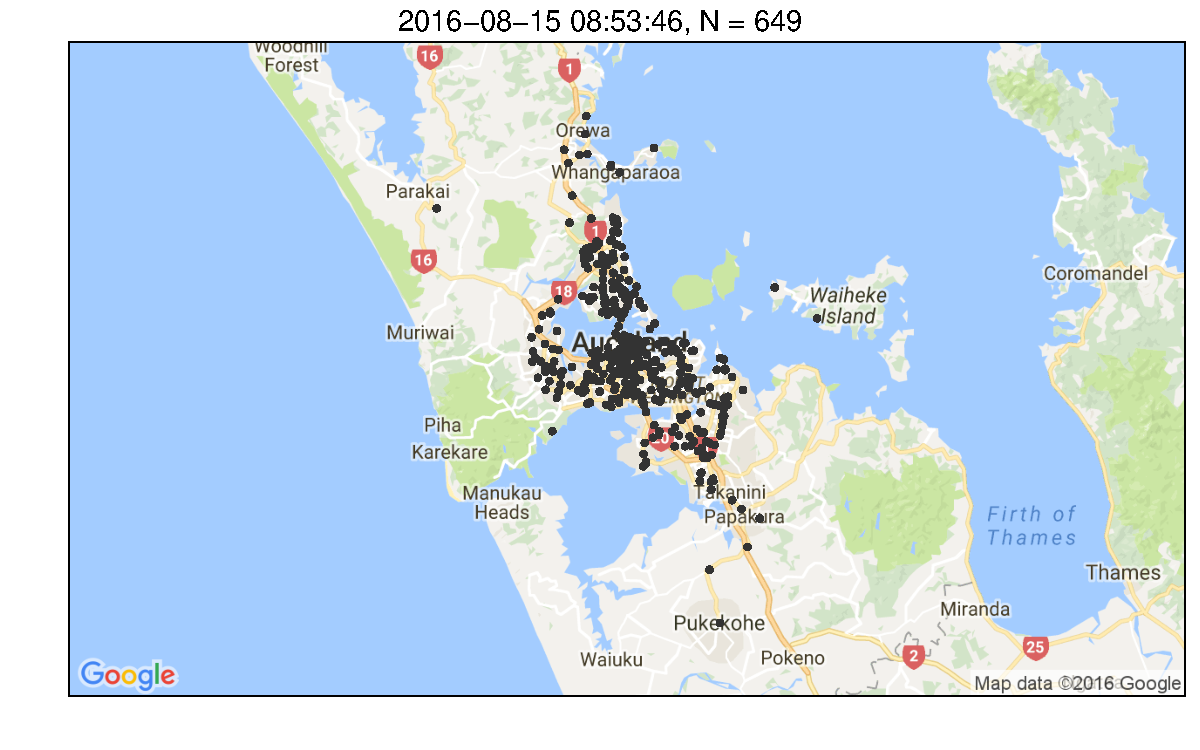
\includegraphics[width=0.8\textwidth,trim={0 0 0 0.6cm},clip]{figure/allbuses.pdf}
  \end{overprint}
\end{frame}


\section{Vehicle State Model}

\begin{frame}
  \frametitle{Vehicle State Model}
  
  \textbf{Goal:} use observations of bus location (GPS) \ldots
  \pause
  \begin{equation*}
    \bY_k = 
    \begin{bmatrix}
      \phi_k \\ \lambda_k \\ t_k
    \end{bmatrix} =
    \begin{bmatrix}
      \text{latitude (degrees)} \\
      \text{longitude (degrees)} \\
      \text{timestamp}
    \end{bmatrix}
  \end{equation*}
  \pause
  \ldots to infer \textbf{unobservable vehicle state} \ldots
  \pause
  \begin{equation*}
    \bX_k =
    \begin{bmatrix}
      d_k \\ v_k \\ s_k \\ \vdots
    \end{bmatrix} =
    \begin{bmatrix}
      \text{distance into trip (meters)} \\
      \text{velocity/speed ($ms^{-1}$)} \\
      \text{last visited stop} \\
      \vdots
    \end{bmatrix}
  \end{equation*}
  \pause
  \ldots in real time.
\end{frame}

\begin{frame}[c]
  \frametitle{Vehicle State Model}
  
  \centering
  \begin{tikzpicture}    
    \node (img1) at (0,0) {\includegraphics{figure/vehicle-state-1.pdf}};
    \node[above of=img1, yshift=2.2cm, xshift=0.3cm] (yk) {$\bY_k$};
    \node[right of=img1,xshift=4cm] (img2) {\includegraphics{figure/vehicle-state-2.pdf}};
    \node[above of=img2, yshift=2.2cm, xshift=1.3cm] (xk) {$\bX_k$ \scriptsize{(first component, $d_k$)}};
  \end{tikzpicture}
  
  \vspace{-1em}
  \scriptsize{Example: Route 274, Britomart to Three Kings}
\end{frame}


\begin{frame}
  \frametitle{Vehicle State Model: Particle Filter}
  
  \begin{itemize}
  \item Represent $\bX_k$ by a \emph{sample} of point-estimates (particles) $\bxi_k$
    
  \item Flexible modeling framework, fewer assumptions
    
  \item Better coverage of possible states (\textbf{multimodality})
    
  \item Intuitive likelihood function
  \end{itemize}
  
  
  \pause
  \textbf{Step 1: predict}
  
  %$\Rightarrow$ independently predict each particle 
  
  %$\Rightarrow$ sample of plausible vehicle states
  
  $\Rightarrow$ generate sample of possible vehicle states
  
  % \
  
  
  \pause
  \textbf{Step 2: update}
  
  $\Rightarrow$ compare predictions to observation, remove those no longer plausible
  
  
  
  %$\Rightarrow$ compute likelihood of each particle
  
  %$\Rightarrow$ weighted resample (with replacement)
  % \begin{equation*}
  %   \bY_k = h(\bX_k) + e_k
  % \end{equation*}
  % {\small$f$: measurement function; $e_k$ measurement (GPS) error}
\end{frame}


\begin{frame}
  \frametitle{Vehicle State Model: Particle Filter}
  
  \textbf{Step 1: predict}
  
  \onslide<+->
  \begin{itemize}
  \item<+-> Start with ``known'' vehicle state, $\bX_{k-1} = \{\bxi_{k-1} : i=1, \ldots, N\}$
    
  \item<+-> \textbf{Transition} each particle independently
    \begin{equation*}
      \bxi_k = f(\bxi_{k-1}, \alert<4>{\sigma_v^2}, \ldots)
    \end{equation*}
    
    \begin{enumerate}
    \item<+-> Add system noise
      \only<4>{
      \begin{equation*}
        v_k^{(i)} \sim \mathcal{N}_T(v_{k-1}^{(i)}, \alert<4>{\sigma^2_v}),
        \qquad 0 \leq v_k^{(i)} \leq \mathbf{v}_{\text{max}}
      \end{equation*}
      $\mathbf{v}_{\text{max}} \approx$ road speed limit
      }
    \item<+-> Move particles along route \only<5>{(Law of Motion)}
      \only<5-6>{
      \begin{equation*}
        d_k^{(i)} \alt<6->{\alert{\leq}}{=} d_{k-1}^{(i)} + (t_k - t_{k-1}) v_k^{(i)}
      \end{equation*}
      }
    \item<6-> What about intermediate stop(s)?
      \only<7->{
      \begin{itemize}
      \item<7-> Does the particle stop? $p_{s_k}^{(i)} \sim \mathrm{Bernoulli}(\pi_{s_k})$
        
      \item<8-> If so, for how long? $\bar t_{s_k} \sim \mathcal{E}(\tau_{s_k})$
        
      \item<9-> \textbf{Dwell time} $ = p_{s_k}^{(i)} \left(\gamma + \bar t_{s_k}\right)$
        
        {\scriptsize $\gamma$ = minimum dwell time (deccelerate/accelerate, open/close doors)}
        
        {\scriptsize $\bar t_{s_k}$ = passengers on/off}
      \end{itemize}
      }
    \end{enumerate}
  \end{itemize}
  
\end{frame}

\begin{frame}
  \frametitle{Vehicle State Model: Particle Filter}
  
  \textbf{Step 1: predict}\\
  Example ($N = 10$ particles)
  
  \vspace{-1em}
  \begin{overprint}
    \onslide<1>
    \includegraphics{figure/predict-state-1.pdf}
    \onslide<2>
    \includegraphics{figure/predict-state-2.pdf}
    \onslide<3>
    \includegraphics{figure/predict-state-3.pdf}
  \end{overprint}
\end{frame}

\begin{frame}
  \frametitle{Vehicle State Model: Particle Filter}
  
  \textbf{Step 2: update}
  
  \onslide<+->
  \begin{itemize}
   
  \item<+-> Likelihood function 
    \only<1-7>{$\ell(\bY_k | \bx_k^{(i)} \only<4-7>{,\alert<4>{h}} \only<5-7>{,\alert<5>{g}})$}
    \only<3-7>{
    \begin{itemize}
      \only<3-7>{ 
      \item Transform particles onto flat plane
        \begin{equation*}
          \bz_k^{(i)} = \alert<5>{g(}\alert<4>{h(\bxi_k)} \alert<5>{| \bY_k)}
        \end{equation*}
        
        \only<4>{
          \alert{$h$: measurement function} (distance into trip $\rightarrow$ lat/lon)
        }
        \only<5>{
          \alert{$g(\cdot|\bY_k)$: projection}
        
          centered on $\bY_k$,  1~unit = 1~meter in all directions
        }
      }
      
      \only<6-7>{
      \item Bivariate normal likelihood, $g(\bY_k | \bY_k) = \boldsymbol{0}$
        \begin{align*}
          \bY_k | \bz_k^{(i)} \sim \bz_k^{(i)} | \bY_k \sim \mathcal{N}_2 (\boldsymbol{0}, \sigma_y^2 I_2)
          \qquad
          \text{(\scriptsize $\sigma_y^2$ = GPS error)}
        \end{align*}        
      }
      
      \only<7>{
      \item For each particle
        \begin{equation*}
          \ell(\bY_k | \bxi_k, h, g) \propto 
          e^{-\frac{1}{2\sigma^2}\left( (\bz_k^{(i)})^T \bz_k^{(i)} \right)}
        \end{equation*}
      }
    \end{itemize}
    }
    
    \only<8->{
    \begin{equation*}
      \ell(\bY_k | \bxi_k, h, g) \propto 
      e^{-\frac{1}{2\sigma^2}\left( (\bz_k^{(i)})^T \bz_k^{(i)} \right)}
    \end{equation*}
    
    
    \item<8-> Compute weights
      
      \begin{equation*}
        w_i = \frac{\ell(\bY_k | \bxi_k)}{\sum_{j=1}^N \ell(\bY_k | \bx_k^{(j)})}
      \end{equation*}
      
    \item<9-> Weighted resample with replacement
      
      \onslide<10->{$\Rightarrow$ keep particles plausible given data}
      %\onslide<10->{$\Rightarrow$ Cull the imaginary busses that are no longer plausible}
    }
    
  \end{itemize}
\end{frame}

\begin{frame}
  \frametitle{Vehicle State Model: Particle Filter}
  
  \textbf{Step 2: update}
  
  \vspace{-1em}
  \begin{overprint}
    \onslide<1>
    \centering
    \includegraphics{figure/predict-state-3.pdf}
    \onslide<2>
    \centering
    \includegraphics{figure/update-state-1.pdf}
    \onslide<3>
    \centering
    \includegraphics{figure/update-state-2.pdf}
    \onslide<4>
    \centering
    \includegraphics{figure/update-state-3.pdf}
    \onslide<5>
    \centering
    \includegraphics{figure/update-state-4.pdf}
    \onslide<6>
    \centering
    \includegraphics{figure/update-state-5.pdf}
    \onslide<7>
    \centering
    \includegraphics{figure/update-state-6.pdf}
  \end{overprint}
\end{frame}


\section{Road State Model}

\begin{frame}
  \frametitle{Road State Model}
  
  \begin{enumerate}[<+->]
  \item \sout<4>{Particle filter $\Rightarrow$ speed estimates for a given bus}
    
  \item Identify segments of road common to multiple routes
    
  \item Use speed information from \emph{all busses} to estimate
    speed along a given road segment
  \end{enumerate}
\end{frame}

\begin{frame}
  \frametitle{Road State Model}
  
  \begin{enumerate}
  \item[2.] Identify segments of road common to multiple routes
    
    \pause
    $\Rightarrow$ between intersections
  \end{enumerate}
  
  
  \begin{overprint}
    \onslide<2>
    \centering
    \includegraphics{figure/road-state-1.pdf}
    \onslide<3>
    \centering
    \includegraphics{figure/road-state-2.pdf}
  \end{overprint}

    
\end{frame}


\begin{frame}
  \frametitle{Road State Model}
  
  \begin{enumerate}
  \item[3.] Use speed information from \emph{all busses} to estimate
    speed along a given road segment

  \end{enumerate}
  
  \pause
  $\Rightarrow$ \textbf{Kalman filter}
    


  \only<3>{
    \textbf{Road state:} mean speed for all $M$ road segments at time $t_\ell$
    \begin{equation*}
      \bnu_\ell = \left[ \nu_{1\ell}\ \nu_{2\ell}\ \cdots\ \nu_{M\ell} \right]^T
    \end{equation*}
    with associated covariance matrix
    \begin{equation*}
      \Xi_\ell =
      \begin{bmatrix}
        \xi_{1\ell} & 0 & \cdots & 0 \\
        0 & \xi_{2\ell} & \cdots & 0 \\
        \vdots & \vdots & \ddots & \vdots \\
        0 & 0 & \cdots & \xi_{M\ell}
      \end{bmatrix}
    \end{equation*}
  }
  
  \only<4->{
    \begin{itemize}
    \item<4-> no complex model necessary (Normal distribution adequate)
      
    \item<5-> updated using particle filter estimates
      
      \begin{equation*}
        \mathbf{v}_\ell = \bnu_\ell + \mathbf{r}_\ell
      \end{equation*}

      \begin{itemize}
      \item $\mathbf{v}_\ell$: mean speed of particles
      
      \item $\mathbf{r}_\ell \sim \mathcal{N}(0, \mat{R}_\ell)$, $\mat{R}_\ell$: variance of particle speeds
      \end{itemize}

    \end{itemize}
  }

\end{frame}

% \begin{frame}
%   \frametitle{Road State Model: Kalman Filter}
  
%   \textbf{Step 1: predict}
%   \begin{equation*}
%     \bnu_\ell = \bnu_{\ell-1} + \bw_\ell
%   \end{equation*}
%   $\bw_\ell \sim \mathcal{N}(0, \mat{Q}_\ell)$: process noise,
%   $\mat{Q}_\ell = (t_\ell - t_{\ell - 1}) \sigma^2_\nu I_M$
  
%   $\sigma^2_\nu = $ segment speed variability 
  
%   \vspace{1em}
%   \pause
%   \textbf{Step 2: update}
%   \begin{equation*}
%     \mathbf{v}_\ell = \bnu_\ell + \mathbf{r}_\ell
%   \end{equation*}
  
%   $\mathbf{r}_\ell \sim \mathcal{N}(0, \mat{R}_\ell)$: measurement error
  
%   $\mathbf{v}_\ell$, $\mathbf{R}_\ell$ estimated using mean and variance of particles
% \end{frame}

% \begin{frame}
%   \frametitle{Road State Model: Kalman Filter}
  
%   \textbf{Step 1: predict}
%   \pause
%   \begin{equation*}
%     \bnu_\ell = \only<4->{I_M}\only<1-3>{\alert<3>{\mat{A}}} \bnu_{\ell-1} + \alert<5>{\bw_\ell}
%   \end{equation*}
%   \pause
%   $\mat{A}$: \alert<3>{transition matrix} \pause $\Rightarrow$ Identity matrix $I_M$
  
%   \pause
%   $\bw_\ell \sim \mathcal{N}(0, \mat{Q}_\ell)$: \alert<5>{Gaussian process noise},
%   $\mat{Q}_\ell = (t_\ell - t_{\ell - 1}) \sigma^2_\nu I_M$
  
%   \vspace{1em}
%   \pause
%   \textbf{Step 2: update}
%   \pause
%   \begin{equation*}
%     \alert<11>{\mathbf{v}_\ell} = 
%     \only<9->{I_M}\only<7-8>{\alert<8>{\mat{H}}}\bnu_\ell + \alert<10>{\mathbf{r}_\ell}
%   \end{equation*}
%   \pause
%   $\mat{H}$: \alert<8>{measurement matrix} \pause $\Rightarrow$ Identity matrix $I_M$
  
%   \pause
%   $\mathbf{r}_\ell \sim \mathcal{N}(0, \alert<12>{\mat{R}_\ell})$: \alert<10>{measurement error}
  
%   \pause
%   \begin{itemize}[<+- | alert@+>]
%   \item $\mathbf{v}_\ell$: mean speed of all particles from $t_{\ell-1}$ to $t_\ell$
    
%   \item $\mat{R}_\ell$: estimated from variance of particles
%   \end{itemize}
  
%   \onslide<+->
%   Standard Kalman filter algorithm to obtain $\bnu_\ell$ and $\Xi_\ell$.
  
% \end{frame}


\section{Predicting Arrival Time}

\begin{frame}
  \frametitle{Predicting Arrival Time}
  
  
  \begin{enumerate}
  \item Schedule
  \item Schedule deviation (AT?)
  \item Vehicle state
  \item Road state
  \end{enumerate}

  % \pause
  % \alert<2>{3.\ and 4.\ include dwell time models}
  
  \pause
  Some notation:
  \begin{itemize}
  \item $S_j^t = $ scheduled arrival time at stop $j$
  \item $\hat A_j = $ (predicted) arrival time at stop $j$
  \item $\tilde T_{s_k}^a, \tilde T_{s_k}^d = $ observed arrival/departure delay at last stop\\
    (from Auckland Transport's API)
  \end{itemize}
 
\end{frame}

\begin{frame}
  \frametitle{Prediction Arrival Time}
  
  \textbf{1. Schedule}
  
  \begin{itemize}    
  \item $\hat A_j = S_j^t$
    
  \item Baseline for other predictors
  \end{itemize}
\end{frame}


\begin{frame}
  \frametitle{Prediction Arrival Time}
  
  \textbf{2. Schedule deviation}
  
  \begin{itemize}    
  \item $\hat A_j = 
    \begin{cases}
      S_j^t + \tilde T_{s_k}^d & \text{ if departed stop $s_k$}\\
      S_j^t + \tilde T_{s_k}^a & \text{ if not departed stop $s_k$}
    \end{cases}$
    
  % \item Sensitive to delays
    
  % \item Unable to incorporate intermediate uncertainty
    
  \item \textbf{OR} use particle estimates of arrival/departure delay, 
    $\tilde A_{s_k}^{(i)}$ and $\tilde D_{s_k}^{(i)}$
  \end{itemize}
\end{frame}

\begin{frame}
  \frametitle{Prediction Arrival Time}
  
  \textbf{3. Vehicle state}
  
  \begin{itemize}[<+->]
    \item $S_j^d = $ distance along route of stop $j$
      
      
    \item $\hat A_j\only<3->{\alert<3>{^{(i)}}} = 
      t_k + \frac{S_j^d - d_k\only<3->{\alert<3>{^{(i)}}}}{v_k\only<3->{\alert<3>{^{(i)}}}}
      \only<4->{\alert<4>{+ \sum_{\ell = s_k+1}^{j-1} p_\ell^{(i)}(\gamma + \bar t_\ell^{(i)})}}$
      
    \item Prediction for each particle
      
    \item Allow for dwell time uncertainty
      
    \item Potentially multi-modal
  \end{itemize}
\end{frame}

\begin{frame}
  \frametitle{Prediction Arrival Time}
  
  \textbf{4. Road state}
  
  \begin{itemize}[<+->]
    \item $r_k = $ route segment index\\
      $R_b = $ distance along route of start of segment $b$
      
    \item $\hat A_j\only<6>{\alert<6>{^{(i)}}} = 
      t_k + \only<3->{\alert<3>{ \frac{R_{s_k\only<6->{\alert<6>{^{(i)}}}+1} - d_k\only<6->{\alert<6>{^{(i)}}}}{\nu_{s_k\only<6->{\alert<6>{^{(i)}}}}} }+} 
      \only<4->{\alert<4>{ \sum_{b\in B^\star} \frac{R_{b+1}-R_b}{\alt<6->{\alert<6>{v_b^{(i)}}}{\nu_b}}  }+}
      \only<5->{\alert<5>{ \frac{S_j^d - R_{b'}}{\alt<6->{\alert<6>{v_{b'}^{(i)}}}{\nu_{b'}}} }}
      \only<7->{\alert<7>{\linebreak\phantom{A_j = }\alert<6>{+ \sum_{\ell = s_k+1}^{j-1} p_\ell^{(i)}(\gamma + \bar t_\ell^{(i)})}}}$
      
    \only<3>{
    \item travel time until end of current segment
    }
    \only<4>{
    \item travel time through intermediate segments ($B^\star$)
    }
    \only<5>{
    \item travel time along segment $b'$ to stop $j$
    }
  \item<6-> For each particle, sample $v_b^{(i)} \sim \mathcal{N}(\nu_b, \xi_b)$
  \item<7-> Allow for dwell time uncertainty
    
  % \item<8-> Uses most recent data
    
  % \item<9-> Opportunity to extend model (e.g., changes in speed over time)
  \end{itemize}
\end{frame}


\begin{frame}
  \frametitle{Predicting Arrival Time}
    
  %\animategraphics{1}{figure/prediction_example_}{01}{39}

  \foreach \x in {1,2,...,8} {
    \only<\x>{
      \includegraphics{figure/prediction_example_0\x.pdf}
    }
  }
  \foreach \x in {9,10,...,38} {
    \pgfmathsetmacro\result{\x + 1}
    \pgfmathtruncatemacro{\xi}{\x + 1}
    \only<\x>{
      \includegraphics{figure/prediction_example_\xi.pdf}
    }
  }


\end{frame}

\begin{frame}
  \frametitle{Predicting Arrival Time}
  
  Conclusions:
  \begin{itemize}[<+->]
  \item \textbf{Schedule:} \ldots
    
  \item \textbf{Schedule deviation:} OK for very short-range prediction; relies on time table accuracy
    
  \item \textbf{Vehicle state:} high variability; OK for short-range prediction
    
  \item \alert<5->{\textbf{Road state:} little variability; performs well at long-range prediction}
  \end{itemize}
  
\end{frame}

\begin{frame}
  \frametitle{Predicting Arrival Time: Intervals}
  
  How do we communicate estimate + uncertainty to commuters?
  
  \onslide<3->{$\Rightarrow$ \textbf{Prediction intervals}}
  \begin{itemize}
  \item<4-> easy to compute from particle sample
    
  \item<5-> intuitive: ETA 6~min (mean) versus ETA 3--8~min
    
  \item<6-> Biased to reduce chance of missing bus
  \end{itemize}
  
  \begin{overprint}
    \onslide<1>
    \centering
    \includegraphics{figure/eta-pred-1.pdf}
    \onslide<2>
    \centering
    \includegraphics{figure/eta-pred-2.pdf}
    \onslide<3->
    \centering
    \includegraphics{figure/eta-pred-3.pdf}
  \end{overprint}
\end{frame}

\begin{frame}
  \frametitle{What's Next?}
  
  \onslide<+->
  \begin{itemize}[<+->]
  \item Add more routes
    
  %\item Incorporate $\tilde T_j^a$/$\tilde T_j^d$ into likelihood
    
  %  $\Rightarrow$ depending on it's reliability
    
  \item Collect historical data to estimate parameters
    \begin{itemize}
    \item Dwell times and stopping probabilties
    \item Segment speed covariance matrix (including off-diagonals)
    \end{itemize}
    
  \item Scale up: \emph{ALL routes/busses} $\Rightarrow$ computational speed
    
  \end{itemize}
\end{frame}


\begin{frame}[standout]
  Thank you!
\end{frame}

\begin{frame}[standout]
  Questions?
\end{frame}

\end{document}
